\clearpage
\section{3 ДАЛЬНЕЙШЕЕ РАЗВИТИЕ РЕАЛИЗАЦИИ}
В ходе реализации упрощённой системы были выявлены следующие технические проблемы, на решение которых необходимо обратить внимание при реализации полной версии:
\begin{itemize}
    \item задача разбиения графа;
    \item ограничение размера мешлетов;
    \item организация параллельной децимации.
\end{itemize}

\subsection*{Задача разбиения графа}
Основной проблемой при реализации является задача разбиения графа.
Эта задача является NP-трудной, для неё не доказано даже вхождение в класс NP.
Из-за этого алгоритмы в библиотеке METIS, как и любые приемлемые алгоритмы в любой другой библиотеке, вычисляют только приближение решения.
Это приводит к значительной неравномерности разбиения, как на рисунке~\ref{fig:sphere-0}.
\begin{figure}[H]
    \centering
    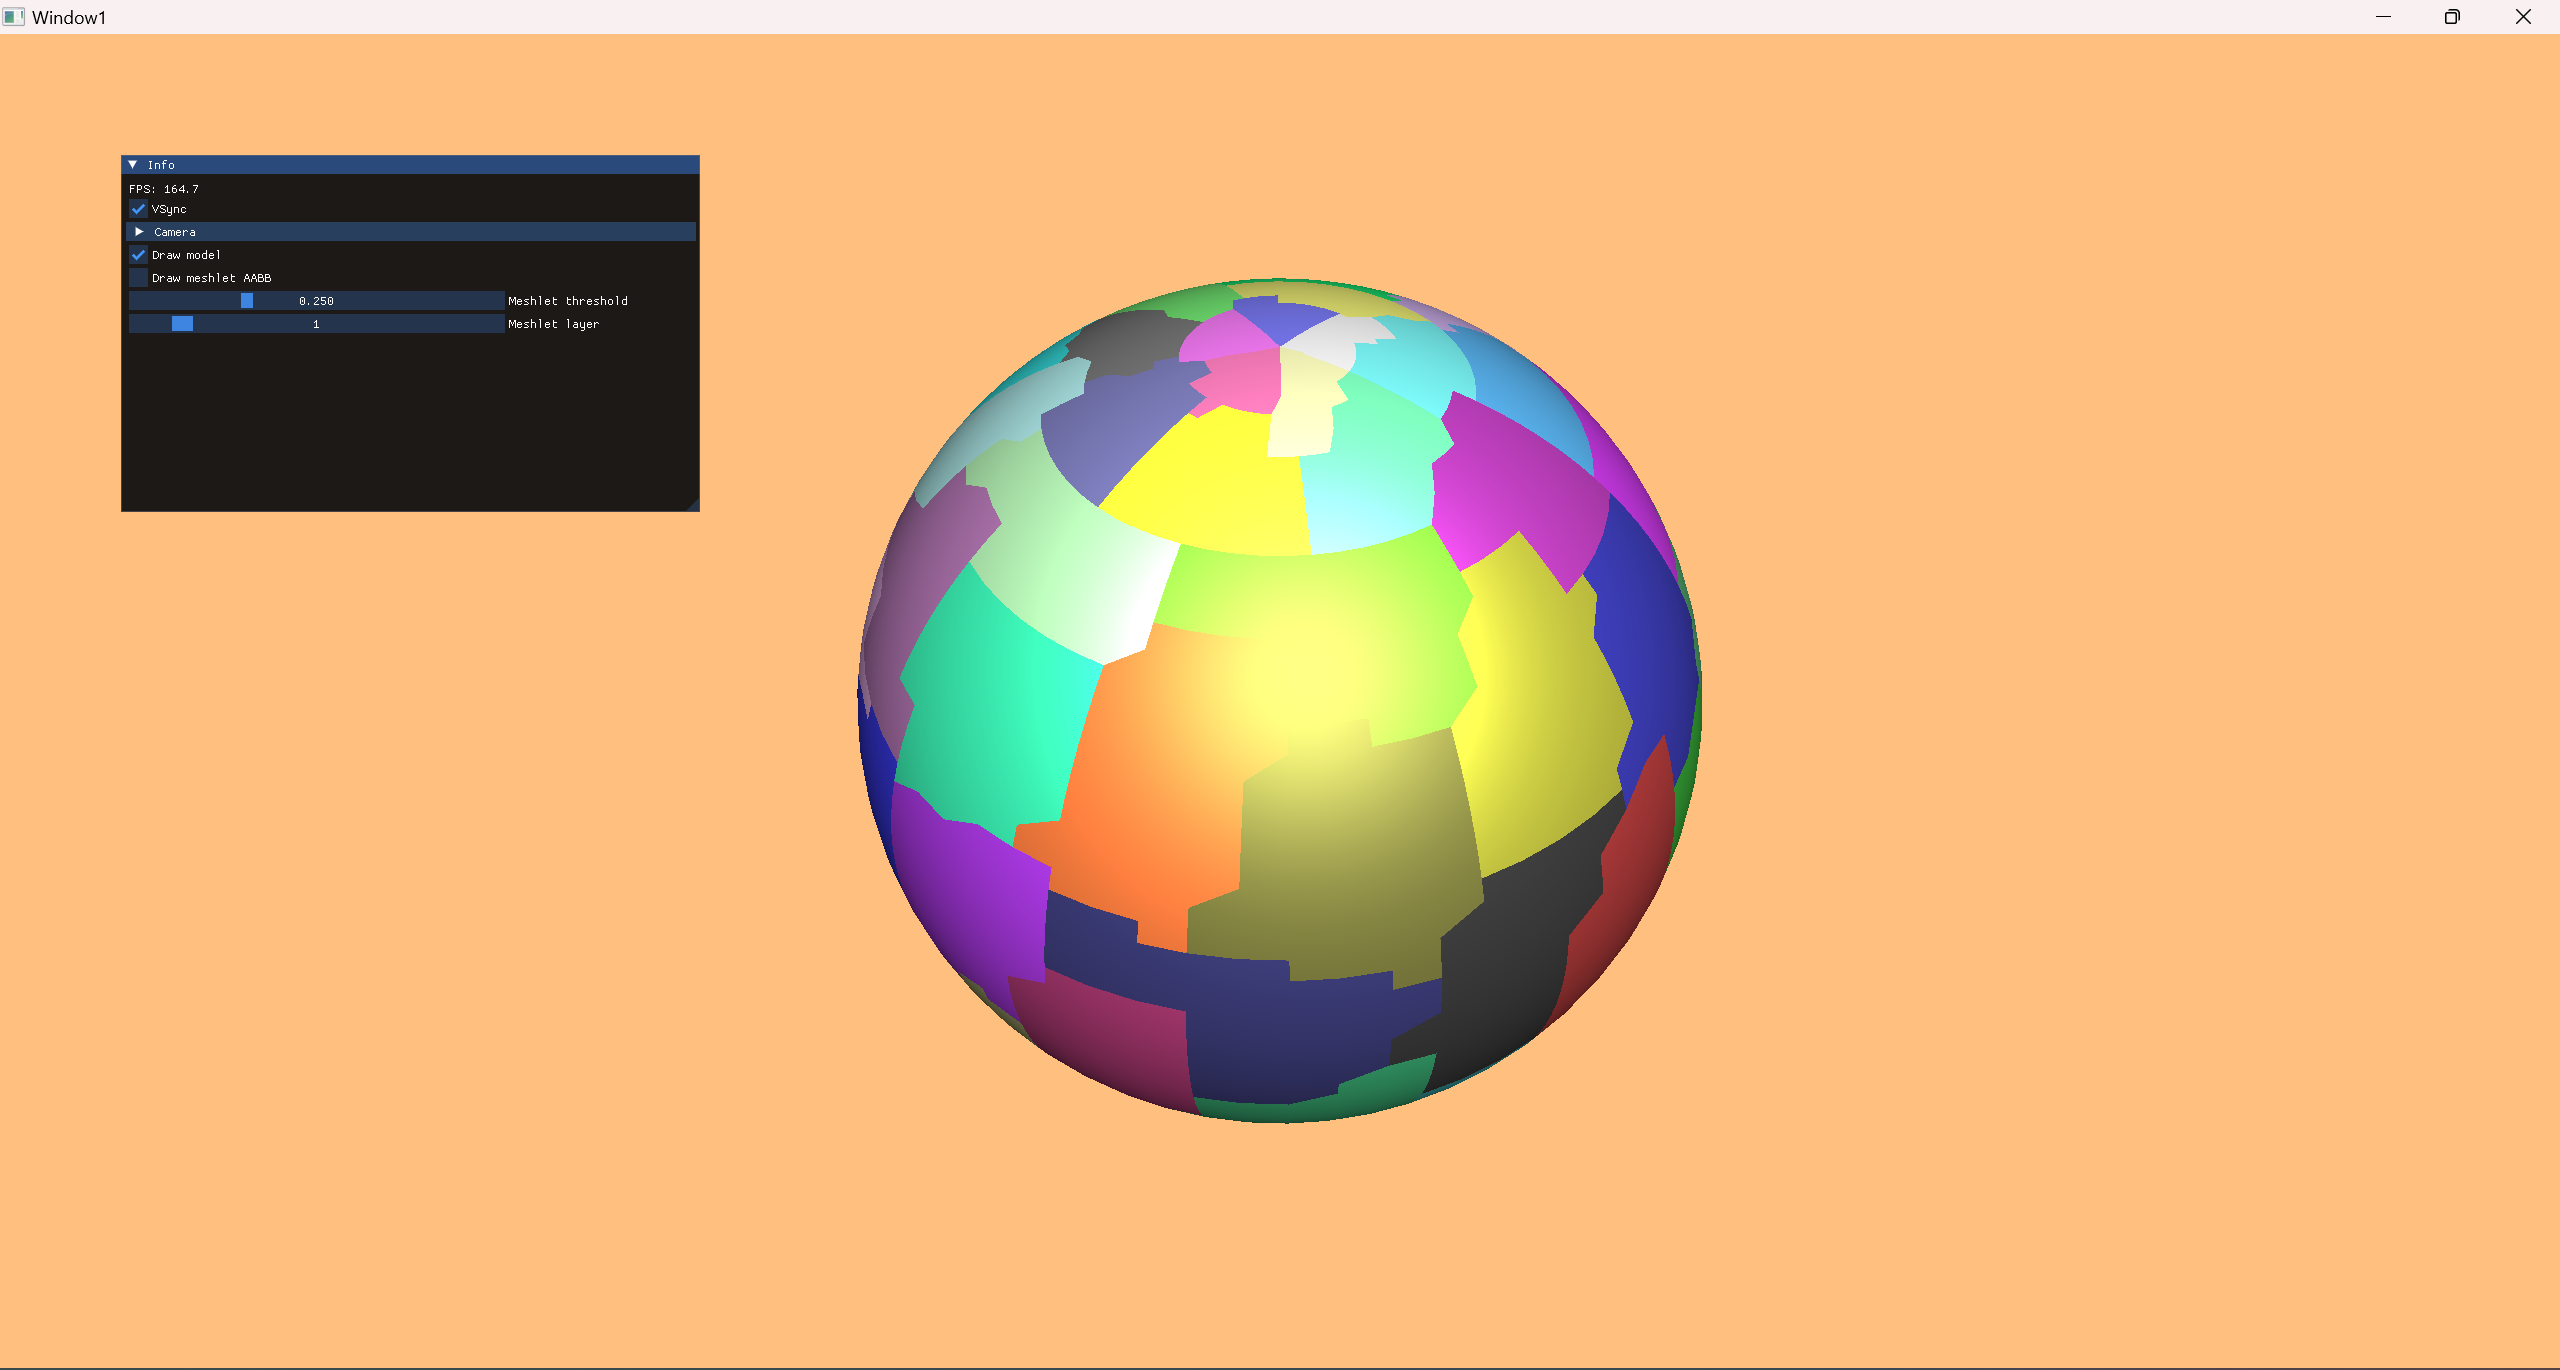
\includegraphics[width=\textwidth]{pics/sphere0.png}
    \caption{Неравномерность разбиения}
    \label{fig:sphere-0}
\end{figure}

Такая неравномерность разбиения, из-за необходимости сохранять швы при децимации, приводит к неравномерности искажений, которые можно наблюдать на рисунке~\ref{fig:sphere-1}.
Эта неравномерность искажений может быть заметна глазу при взгляде на изначально симметричные объекты.
\begin{figure}[H]
    \centering
    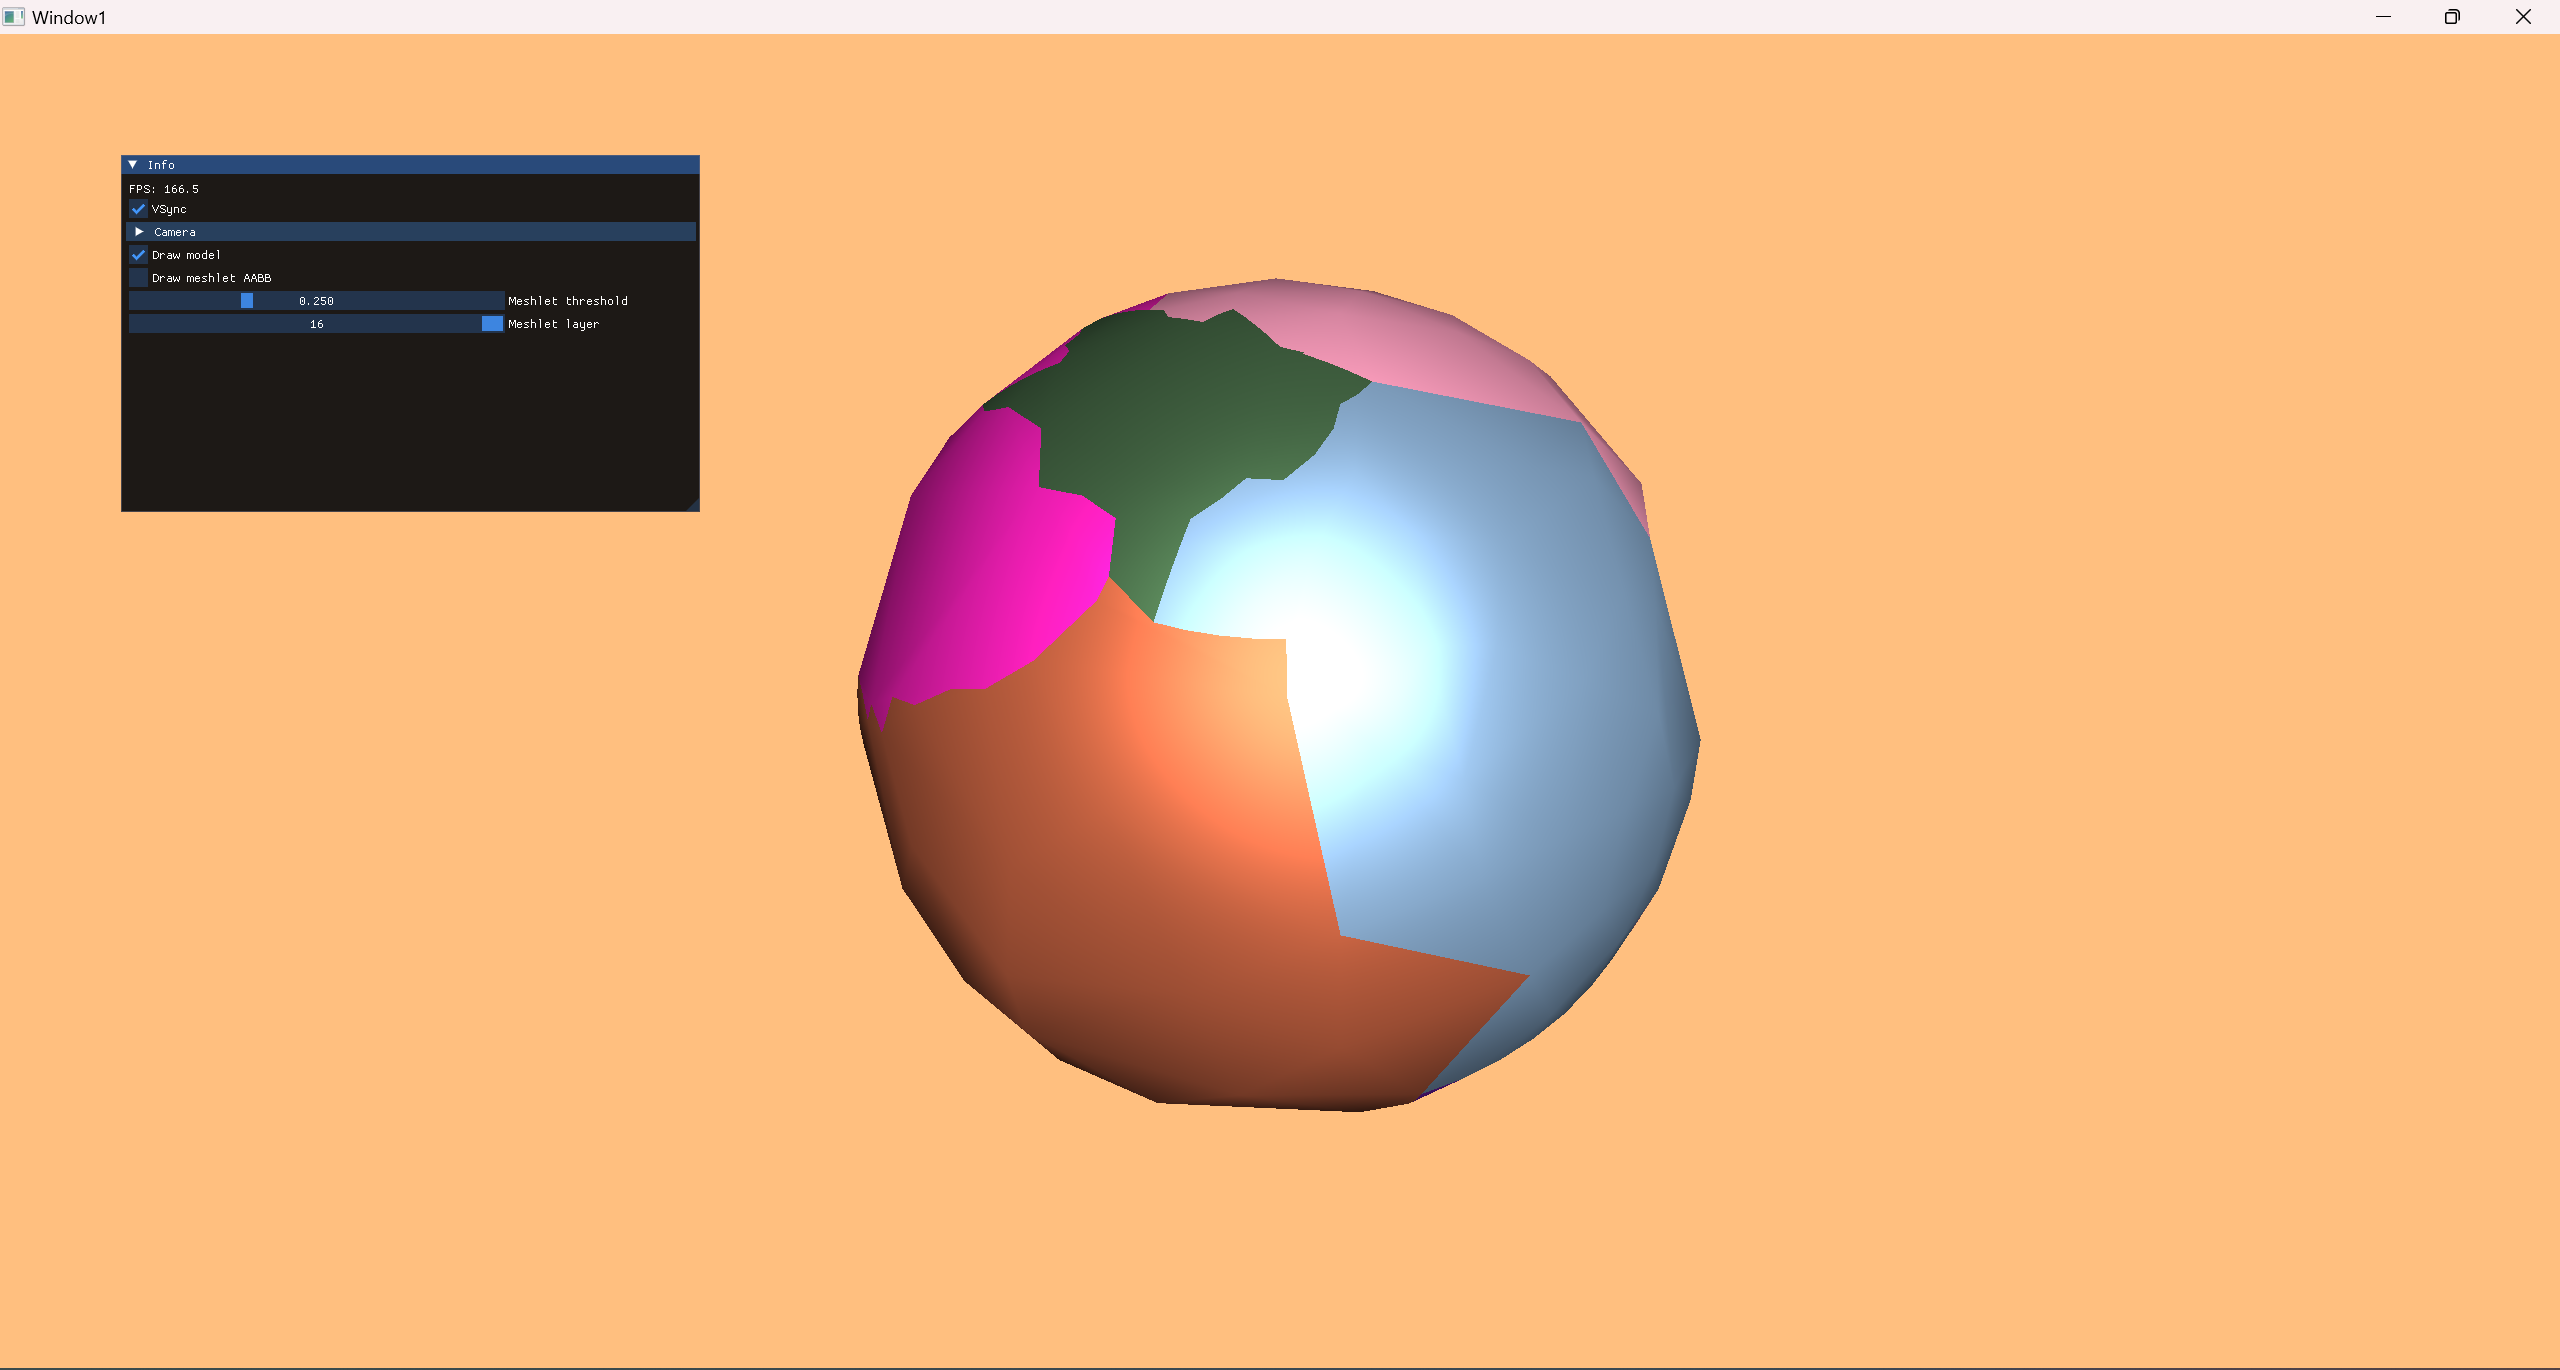
\includegraphics[width=\textwidth]{pics/sphere1.png}
    \caption{Неравномерность искажений}
    \label{fig:sphere-1}
\end{figure}

\subsection*{Ограничение размера мешлетов}
Другой заметной технической проблемой является ограничение размера мешлетов при разбиении графа.
Mesh Shader позволяет использовать мешлеты размером не более 256 вершин и 256 примитивов, это обусловлено механизмом работы общей для группы потоков памяти.
Поскольку METIS не позволяет задать это ограничение, приходится использовать неоптимальное количество мешлетов.

NVidia рекомендует использовать размер мешлета в 64 вершины и 126 треугольников, в то же время размер мешлета на выходе METIS является случайной величиной.

\subsection*{Огранизация параллельной децимации}
В рамках выпускной квалификационной работы децимация супермешлетов производится в однопоточном режиме.
В результате этого время обработки оказывается значительным: для тестового меша размером 10 млн. треугольников время предподсчёта составило 170 минут на процессоре AMD Ryzen 7 5700H, процессу потребовалось 6 ГБ памяти.
